\chapter*{Bitcoin cryptocurrency study}
\addcontentsline{toc}{chapter}{Bitcoin cryptocurrency study}
\label{chap:bitcoin_study}
Following our tutor's recommendation, we started to study the concept and operation of the Bitcoin cryptocurrency and network using a breadth-first strategy. We started with the basic concepts (mainly cryptographical tools and techniques) about Bitcoin. Then, we studied the main concepts and ideas about how transactions are performed, blocks are created, and consensus is reached at a high level. 

Finally, we started to research how all concepts are used in detail, by understanding the current Bitcoin protocol implementation byte per byte (focusing just on everything related to transactions, that will allow us to create the payment channels)

\section{The goals}
As the main goal for this stage of study and research, we had to understand at a byte level how a Bitcoin transaction is constructed, therefore understanding also the Bitcoin scripting language

\section{The basics about Bitcoin}
To understand how Bitcoin works, we enrolled in a \textit{MOOC}, a coursera course recommended by our tutor\cite{bitcoin_coursera:online}. In these course, we reviewed the tools and techniques, mainly cryptographical needed in order to have the main knowledges to understand Bitcoin, that we already learnt in previous University subjects. After that, a global vision of the idea of cryptocurrency and how Bitcoin puts it in practice is explained and later detailed a little bit more technically but without getting into implementation details. Politics, cryptocurrency and other subjects were skipped as didn't contribute any relevant information to our project. With these course finished, we accomplished the first tasks of learning the Bitcoin basics.

\section{Bitcoin low-level understanding}
Despite there are quite a lot sites with information about the Bitcoin cryptocurrency, the fact is that when dealing with Bitcoin in a low-level detail, information is scarcely found. Most of the information to understand the Bitcoin protocol implementation was found in a Wiki-like site called \textit{Bitcoin.it}\cite{bitcoin_wiki:online}. The rest of information was found in developer Q\&A sites like \textit{StackOverflow}\footnote{\url{https://stackoverflow.com}} or the more Bitcoin-specific site \textit{Bitcoin Stack Exchange}\footnote{\url{https://bitcoin.stackexchange.com/}}, and several forums and blogs (that will be properly cited in the report in the following pages and are also properly cited in the software code documentation)

\section{Transaction low-level understanding}
Once we understood how basic concepts were implemented in the Bitcoin protocol, we decided to take sample pay to public key address transactions from the main Bitcoin network (also known as the production network), as most of them are of that kind and regular (we could be unlucky and pick strange transactions from the \textit{testnet}, the development Bitcoin network used for new features testing).

We chose to understand low-level, byte per byte, pay to public key address transactions first as they are the most simple transactions: they spend funds by signing using a private key and send funds by specifying (the hash of) a public key. We have to understand fully the most simple transactions to create complexer transactions with specific spend and payment conditions (also called \textit{smart contracts})

We studied the meanings and the encodings used (little endian most of them) of all the fields in a transaction and compared our knowledge with real transactions we took from the \textit{mainnet} using a block explorer\cite{webbtc:online}\cite{blockr_btc:online}.

The summary is that a Bitcoin transaction contains a version field, inputs field, outputs field, and a locktime field, with each field having a specific byte format and representation. The inputs field contain a list of inputs, where each of them references to the transaction (UTXO, unspent transaction output) that will be spent, its spent script (signatures and public keys in P2PKH cases) and a sequence field. In the case of the outputs, it specifies a list of outputs fields where each output contains a value and a script containing the conditions that the spender must satisfy to spend it (in P2PKH cases, the hash of the public key whose paired private key will sign the spending transaction).


\begin{figure}[H]
The following picture illustrates a low-level transaction and its fields:\\\\
  {\centering
  \makebox[\textwidth]{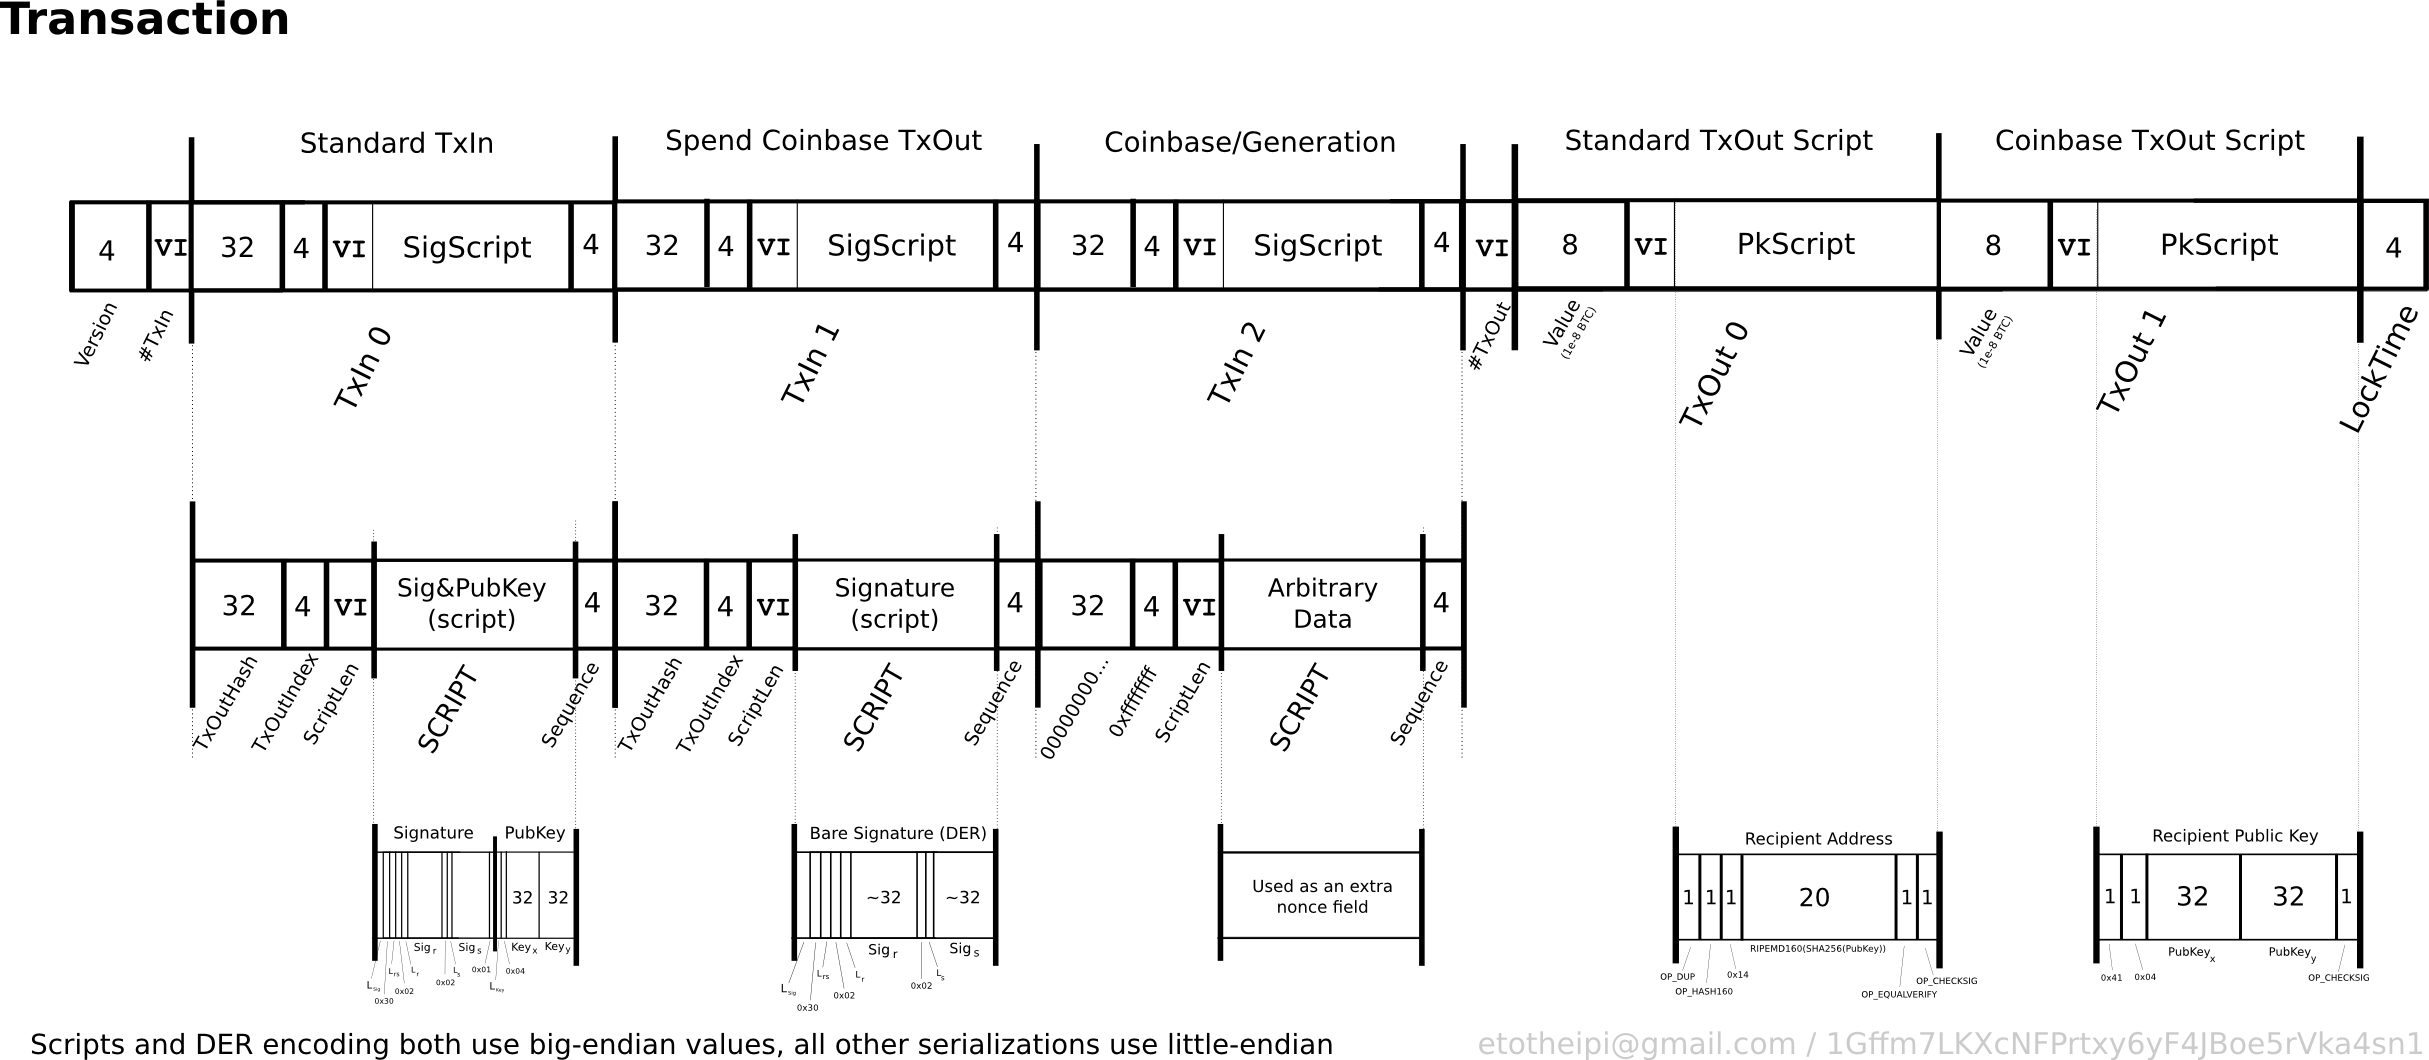
\includegraphics[width=\linewidth]{tx-binary.png}}
  \caption{A Bitcoin transaction in low-level, byte detail\cite{bitcoin_wiki_raw_tx:online}}}
  \label{fig:raw-tx}
\end{figure}

Understanding the version, number of inputs and outputs, references to outputs in inputs and specification of output values was mostly a reading task to know the byte format and encoding from the \textit{Bitcoin Wiki}\cite{bitcoin_wiki_tx:online}. Some fields like \textit{sequence} or \textit{locktime} were not researched depthly as were not relevant in that moment. The most difficult pieces to understand where the scripts, that specify how the transaction outputs can be spend and how the transaction inputs (that point to unspent outputs) get spent. 

\section{Script low-level understanding}
To understand scripts, the \textit{Bitcoin Wiki}\cite{bitcoin_wiki_script:online} provided very useful information about them in low-level, despite omitting (or not specifying clearly) details like the \textit{push data} opcodes. Several posts from forums, blogs and Q\&A answer sites where used to complete the information\cite{siliconian_raw_tx:online, stackoverflow_raw_tx:online}. The most difficult part was to understand how signatures are performed, since a new special transaction (copy of the transaction but removing some fields) has to be created to then sign it and set it into DER format in order to add a signature to a script\cite{bitcoin_wiki_sign:online, stackoverflow_signature_der:online}.

To view scripts in a more graphical way, the online site \textit{WebBTC} provided a visual script executor given a blockchain transaction\cite{webbtc_script:online} and \textit{hashmal} project from \textit{mazaclub} GitHub user provided a GUI to create and test scripts\cite{hashmal:online}.
\begin{figure}[H]
  \centering
  \makebox[\textwidth]{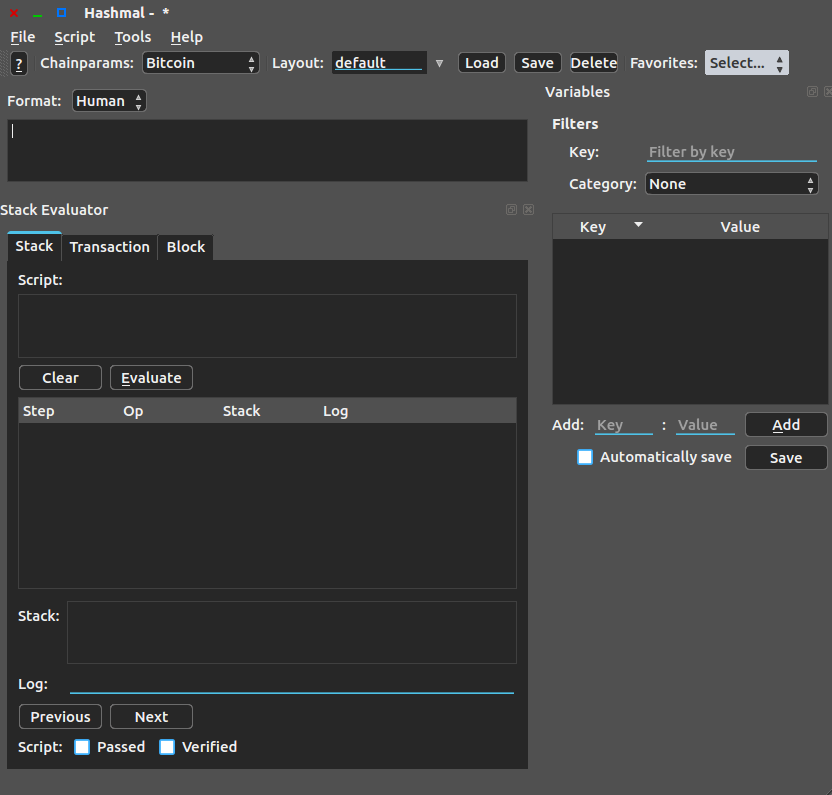
\includegraphics[width=\linewidth]{hashmal.png}}
  \caption{\textit{Hashmal} script editor and executor screenshot}
  \label{fig:hashmal}
\end{figure}

\section{Conclusions about the research}
Once the research was concluded and a raw transaction in bytes had acquired meaning for us, being able to decode most of the bytes in it, we concluded several points:
\begin{itemize}
    \item \textbf{The Bitcoin and \textit{smart contracts} potential}\\
    The fact that Bitcoin allows scripts to set how the funds of a transactions can be spent and scripts to spend those funds providing the conditions specified, has an enormous potential as allows developing \textit{smart contracts} that ables us to perform financial transactions with a huge set of possible spending conditions just limited to the scripting language limits, where those transactions will be protected cryptographically by a decentralized network of nodes that will check and validate that those conditions are accomplished. These idea and its potential has never seen before the appearance of Bitcoin.
    \item \textbf{Sparsed and few low-level documentation}\\ Despite there's quite much information about the Bitcoin concept and high-level operation explanations, there are just few websites that explain how Bitcoin works at a low-level detail, explaining what each byte means inside a transaction. Even best way to understand some details is to look at the Bitcoin Core's C++ implementation\cite{bitcoin_github:online}, the widely used Bitcoin node (with some comments that try to make the code more readable). Developing an informative website or media that collects and explains Bitcoin from the highest to the lowest level would be a really interesting and valuable educational resource that could aim more developers to play with the Bitcoin technology
    \item \textbf{The need for software models and architectures (ie: a framework)}\\ Due to the lots of concepts, ideas and dispersed items that play a role in Bitcoin (and just knowing and fully-understanding the transactions and therefore script pieces), defining a model (an object in OOP) for each item that is present in the process of a transaction generation can be a way to allow faster features development by abstracting hard low-level details so new developers don't get afraid to develop new Bitcoin features without spending hours to understand absolutely everything and losing time with technical, technological, programming-language details that don't provide any value or innovation. We'll try to create those models as much as our timing and project scope allows us to create them without delaying the schedule.\\ In this sense, the alt-currency Ethereum\cite{ethereum:online} has made great progress.
\end{itemize}
